\documentclass[aspectratio=169]{beamer}

\usepackage{amsmath,amssymb}
\usepackage{booktabs}
\usepackage{graphicx}
\usepackage{xcolor}
\usepackage{hyperref}

\usetheme{default}
\setbeamertemplate{navigation symbols}{}
\setbeamertemplate{footline}[frame number]
\definecolor{princetonOrange}{HTML}{E77500}
\definecolor{slate}{HTML}{233142}
\setbeamercolor{title}{fg=slate}
\setbeamercolor{frametitle}{fg=slate}
\setbeamercolor{structure}{fg=princetonOrange}

\title{Polynomial Input Preconditioning for Zero-Shot Time-Series Forecasting}
\author{Jerry Han\\Advisor: Prof. Elad Hazan}
\institute{Program in Statistics and Machine Learning\\Princeton University}
\date{CSML Independent Work, Spring 2026}

\begin{document}

\begin{frame}
  \titlepage
\end{frame}

\begin{frame}{Preliminaries: Universal Sequence Preconditioning}
\large
\begin{itemize}
  \item Marsden and Hazan study online prediction for marginally stable linear dynamical systems.
  \item USP first transforms the observed sequence with a fixed polynomial convolution:
\end{itemize}
\[
  x^{\mathrm{pre}}_t = \sum_{k=0}^{d} a_k x_{t-k}.
\]
\begin{itemize}
  \item Chebyshev-style coefficients are chosen to uniformly damp difficult hidden dynamics.
  \item Intuition: make the visible sequence easier to predict without identifying the hidden state.
  \item This project tests whether that fixed preconditioning signal also helps patch-based transformers.
\end{itemize}
\end{frame}

\begin{frame}{Problem: patching creates an early bottleneck}
\large
\begin{itemize}
  \item Moirai 2.0 splits a time series into fixed-length patches.
  \item Each patch is embedded independently before attention.
  \item Cross-patch structure must be discovered later inside the transformer.
\end{itemize}
\vspace{0.25in}
\begin{center}
\textbf{Question:} can a fixed polynomial signal expose useful structure before tokenization?
\end{center}
\end{frame}

\begin{frame}{Method: add one fixed polynomial channel}
\large
\[
  r_t = \sum_{k=1}^{d} c_k x_{t-ks}
\]
\[
  d=4,\quad s=P=16,\quad r_t=-x_{t-32}+\frac{1}{8}x_{t-64}
\]
\vspace{0.08in}
\begin{itemize}
  \item Concatenate $[\text{input patch};\text{mask};\text{residual patch}]$.
  \item Widen only the input projection: $2P \to 3P$.
  \item Transformer decoder and forecast target are unchanged.
  \item Overhead: 12K parameters, or 0.11\%.
\end{itemize}
\end{frame}

\begin{frame}{Architecture}
\begin{center}

\includegraphics[width=0.95\linewidth]{../figures/fig_architecture.pdf}
\end{center}
\end{frame}

\begin{frame}{Main result: GIFT-Eval}
\begin{center}
\large
\begin{tabular}{lccc}
\toprule
Method & MASE & $\Delta$ & Wins \\
\midrule
\textbf{\texttt{d4\_dropout}} & \textbf{0.837} & \textbf{$-2.9\%$} & \textbf{72/97} \\
\texttt{d4} & 0.838 & $-2.8\%$ & 72/97 \\
Zero control & 0.858 & $-0.5\%$ & 54/97 \\
Baseline & 0.862 & --- & --- \\
Duplicate control & 0.865 & $+0.4\%$ & 39/97 \\
\bottomrule
\end{tabular}
\end{center}
\vspace{0.1in}
\large Paired sign test after averaging across 5 seeds: $p<10^{-5}$.
\end{frame}

\begin{frame}{Ablations and external validation}
\begin{columns}
\begin{column}{0.49\linewidth}
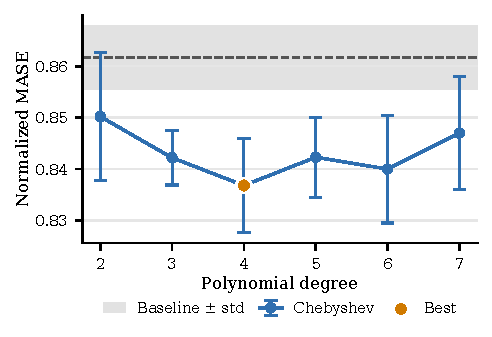
\includegraphics[width=\linewidth]{../figures/degree_sweep_line.pdf}
\end{column}
\begin{column}{0.49\linewidth}
\large
\textbf{FEV-Bench:}
\begin{itemize}
  \item MASE: $-2.91\%$
  \item SQL: $-3.09\%$
  \item Wins: 72/100
\end{itemize}
\vspace{0.1in}
Fixed Chebyshev coefficients beat learned coefficient vectors from both Chebyshev and zero initialization.
\end{column}
\end{columns}
\end{frame}

\begin{frame}{Training dynamics}
\begin{center}
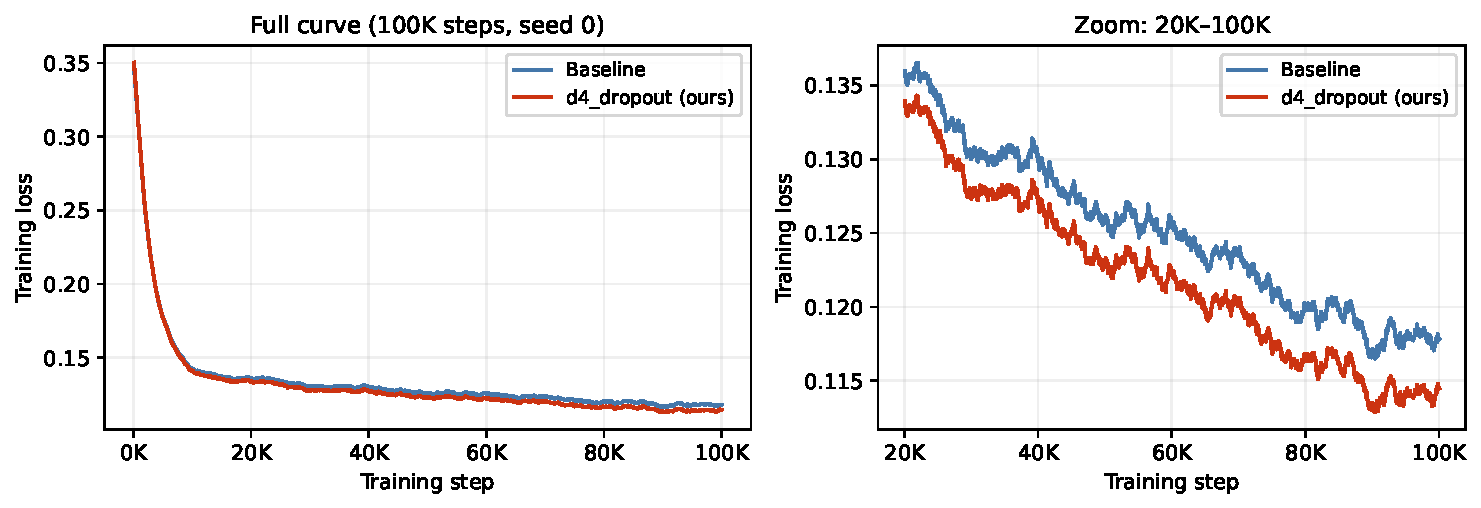
\includegraphics[width=0.82\linewidth]{../figures/fig_training_loss_main.pdf}
\end{center}
\large
At 100K steps, the improvement reaches $-3.9\%$ MASE and cross-seed standard deviation is lower than baseline.
\end{frame}

\begin{frame}{Takeaways}
\large
\begin{itemize}
  \item A fixed Chebyshev input channel improves a modern zero-shot forecaster.
  \item Capacity controls show the gain comes from polynomial content, not added width.
  \item The method is parameter-efficient: 0.11\% overhead and no transformer changes.
  \item This suggests a practical alternative to improving time-series foundation models only by scaling.
\end{itemize}
\end{frame}

\end{document}
